 \chapter{Numerical results for the implicit coupling schemes}

This chapter provides validation and comparison results for the implicit solution schemes.
It focuses on two examples.
The quasi-static finite strain thermo-elastic expansion of an infinitely long-thick walled cylinder and the necking of a thermo-elastoplastic circular bar.

% \section{Second Danilovskaya problem}
%
% The second Danilovskaya problem is proposed in \cite{danilovskaya_dynamical_1952} and it is used frequently in the literature for the validation of a fully coupled thermomechanical model (\cite{farhat_unconditionally_1991}, \cite{tosaka_boundary_1991}, \cite{tamma_effective_1992}, \cite{tanaka_application_1995} and \cite{danowski_computational_2014}).
% Following the description in \cite{danowski_computational_2014}, the geometry is in the form of a cuboid of height and width equal to \SI{4}{\milli\meter} and a length of \SI{6}{\milli\meter}, as is shown in Figure~\ref{fig:setup_2nd_danilovskaya}.
% The solid is linear elastic and subject to a heat flux on the surface \(x=\SI{0}{\milli\meter}\).
% Here, \(\hat Q_C \equiv \hat q_C\) \jvc{Make notation consistent.} as only small deformation, i.e., \(\mathbf F \equiv \mathbf I\), are considered.
%
% \begin{figure}
%   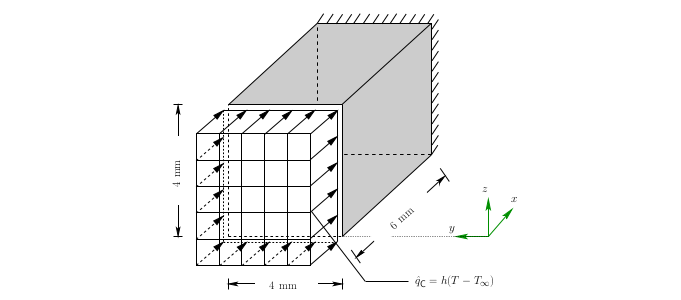
\includegraphics[width=\textwidth]{figures/setup_2nd_danilovskaya.png}
%   \caption{Setup for the second Danilovskaya problem. Initial geometry and prescirbed heat convection boundary condition \(\hat q_C\).}
%   \label{fig:setup_2nd_danilovskaya}
% \end{figure}
%
% The simulation performed in three spatial dimensions.
% However, all displacement degrees of freedom in the \(y\)- and \(z\)-directions are fixed, such that a quasi-one-dimensional motion is produced.
% The body is assumed to be mechanically constrained and thermally insulated.
%
% The mechanical and thermal field properties are given in Table~\ref{tab:snd_danilovskaya_description}, where \(\bar{h}\) denotes the kinematic heat transfer coefficient, defined as \(\bar{h}=\frac{h}{\rho C_V}\) with the linear heat transfer coefficient \(h\).
% Furthermore, the values for the thermal conductivity \(k\), the coefficient of thermal expansion \(\alpha_{T}\), the constant initial temperature \(T_{0}\), as well as an ambient temperature \(T_{\infty}\) are given.
% The elastic constants characterizing the material are the Young's modulus \(E\) and Poisson's rate \(v\).
% A linear thermoelastic material is chosen according to the model described in \cite{armero_new_1992}.
%
% In the literature (\cite{farhat_unconditionally_1991}, \cite{tosaka_boundary_1991}, \cite{tamma_effective_1992}, \cite{tanaka_application_1995}), the density \(\rho\) and the heat capacity \(C_V\) are not divulged, and can in theory, be chosen arbitrarily according a dimensionless termomechanical parameter \(\delta\).
% However, to achieve a direct comparison with the results in \cite{tanaka_application_1995}, \cite{danowski_computational_2014} chose after calibration \(\rho=\SI{7.850}{\kilo\gram\meter^{-3}}\), yielding \(C_V = \SI[exponent-mode=engineering]{0.821}{\joule\kg^{-1}\kelvin^{-1}}\).
% These values are adopted here as well.
%
% \begin{table}
%   \centering
%   \caption{Material properties, and initial and boundary conditions for the second Danilovskaya problem.}
%   \label{tab:snd_danilovskaya_description}
%   \begin{tabular}{ccS[exponent-mode=engineering]}
%   \multicolumn{2}{c}{Material Properties} & {\vphantom{\Big |}Effective value}\\
%   \hline\hline
%   \vphantom{\Big |}Density \(\rho\) & (\si{\newton\second^2\milli\meter^{-4}}) & 7850e-12\\
%   \vphantom{\Big |}Young's modulus \(E\) & (\si{\newton\milli\meter^{-2}}) & 210e3\\
%   \vphantom{\Big |}Poisson's coefficient \(\nu\) & - & 0.3\\
%   \vphantom{\Big |}Conductivity \(k\) & (\si{\newton\second^{-1}\kelvin^{-1}}) & 1.03\\
%   \vphantom{\Big |}Heat capacity \(C_V\) & (\si{\milli\meter^2\second^{-2}\kelvin^{-1}}) & 0.821e6\\
%   \vphantom{\Big |}\makecell[c]{Coefficient of\\ thermal expansion} \(\alpha_T\) & (\si{\kelvin^{-1}}) & 1.1e-6\\
%   \hline
%   \multicolumn{2}{c}{Boundary Conditions\vphantom{\Big |}} & \\\hline
%   \vphantom{\Big |}Dimension \(l_x\) & (\si{\milli\meter}) & 6\\
%   \vphantom{\Big |}Dimension \(l_y\) & (\si{\milli\meter}) & 4\\
%   \vphantom{\Big |}Dimension \(l_z\) & (\si{\milli\meter}) & 4\\
%   \makecell[c]{Kinetic heat\\ convection coefficient} \(\bar h\) & (\si{\milli\meter\second^{-1}}) & 100e-3\\
%   \multicolumn{3}{c}{\vphantom{\Big |}All mechanical degrees of freedom fixed in the \(y\)- and \(z\)-directions.}\\
%   \hline
%   \multicolumn{2}{c}{Initial Conditions\vphantom{\Big |}} & \\\hline
%   \vphantom{\Big |}Ambient temperature \(T_\text{env}\) & (\si{\kelvin}) & {373.15}\\
%   Intial temperature \(T_0\) & (\si{\kelvin}) & {273.15}\\
%   \hline
%   \multicolumn{2}{c}{Reference value \vphantom{\Big |}} & \\\hline
%   \vphantom{\Big |}Temperature at point \(E\) (\(x=\SI{1}{\milli\meter}\)) & (\si{\kelvin}) & \\
%   \hline\hline
%   \end{tabular}
% \end{table}
%
% The discretisation for both the mechanical and thermal field contains each \(n_{x} \times n_{y} \times n_{z}=12 \times\) \(4 \times 4\) Hex 8 elements.
% The simulation time is \(t=\SI{4}{\second}\), with a time-step size of \(\Delta t=\SI{0.001}{\second}\).
% Moreover, a one-step- \(\theta\) time integration is chosen with the value \(\theta=0.5\), resulting in a CrankNicolson scheme for the temperature field, and quasi-static approach for the mechanical field.
% Displacements and temperatures are evaluated at the centre point of the plane at \(x=\SI{1}{\milli\meter}\).

\section{Expansion of a thermoelastic thick-walled cylinder}

The following numerical example concerns the quasi-static finite strain thermo-elastic expansion of an infinitely long thick-walled cylinder, as presented in \cite{ibrahimbegovic_thermodynamics_2009}.
\cite{armero_new_1992} and \cite{erbts_accelerated_2012} also present results regarding this problem, although the dimensions of the cylinder considered there are different from the ones used in the present work.
Linear quadratic elements (QUAD4) are used in the FEM discretization employed.
Thanks to the axial symmetric of the problem, only one-fourth of the cylinder is considered with an inner radius of \(r_{0}=5 \mathrm{~mm}\) and an outer radius of \(r_{1}=15 \mathrm{~mm}\), as depicted in Figure~\ref{fig:fem_discretization}.
All material properties and model properties can be found in Table~\ref{tab:expansion_thick_walled_cylinder}.

\begin{figure}
  \centering
  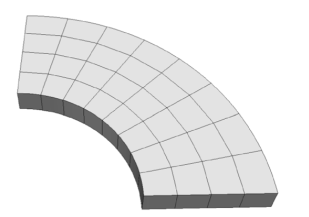
\includegraphics[width=0.5\textwidth]{fem_discretization}
  \caption{Infinitely long thick-walled cylinder whose quasi-static finite strain thermo-elastic expansion, including the FEM discretization employed.}
\label{fig:fem_discretization}
\end{figure}

\begin{table}
  \centering
  \caption{Material properties, and initial and boundary conditions for the problem concerning the quasi-static finite strain thermo-elastic expansion of an infinitely long thick-walled cylinder.}
\label{tab:expansion_thick_walled_cylinder}
  \begin{tabular}{ccS[exponent-mode=engineering]}
  \multicolumn{2}{c}{Material Properties} & {\vphantom{\Big |}Effective value}\\
  \hline\hline
  \vphantom{\Big |}Density \(\rho\) & (\si{\newton\second^2\milli\meter^{-4}}) & 7.8e-9\\
  \vphantom{\Big |}Bulk modulus \(\kappa\) & (\si{\newton\milli\meter^{-2}}) & 164206\\
  \vphantom{\Big |}Shear modulus \(\mu\) & (\si{\newton\milli\meter^{-2}}) & 80140\\
  \vphantom{\Big |}Conductivity \(k\) & (\si{\newton\second^{-1}\kelvin^{-1}}) & 45\\
  \vphantom{\Big |}Heat capacity \(C_V\) & (\si{\milli\meter^2\second^{-2}\kelvin^{-1}}) & 460e6\\
  \vphantom{\Big |}\makecell[c]{Coefficient of\\ thermal expansion} \(\alpha_T\) & (\si{\kelvin^{-1}}) & {\SI[exponent-mode=engineering]{0}{} - \SI[exponent-mode=engineering]{1.5e-4}{}}\\
  \hline
  \multicolumn{2}{c}{Boundary Conditions\vphantom{\Big |}} & \\\hline
  \vphantom{\Big |}Inner radius \(r_0\) & (\si{\milli\meter}) & 5\\
  \vphantom{\Big |}Outer radius \(r_1\) & (\si{\milli\meter}) & 15\\
  \vphantom{\Big |}Inner radius rate of displacement \(\dot u_0\) & (\si{\milli\meter\second^{-1}}) & {0.1; 0.25; 0.5}\\
  \vphantom{\Big |}Heat at inner radius \(q_1\) & (\si{\newton\second^{-1}\milli\meter^{-1}}) & 0\\
  \vphantom{\Big |}Temperature outer radius \(T_1\) & (\si{\kelvin}) & 273.15\\
  % \multicolumn{3}{c}{\vphantom{\Big |}All mechanical degrees of freedom fixed in the \(y\)- and \(z\)-directions.}\\
  \hline
  \multicolumn{2}{c}{Initial Conditions\vphantom{\Big |}} & \\\hline
  Intial temperature \(T_0\) & (\si{\kelvin}) & {273.15}\\
  \hline
  \multicolumn{2}{c}{Reference value \vphantom{\Big |}} & \\\hline
  \vphantom{\Big |}Temperature at inner radius (\(r=r_0\)) & (\si{\kelvin}) & \\
  \hline\hline
  \end{tabular}
\end{table}

% The displacement and the heat flux in the axial direction are restricted to zero, \(u_{z}=0\) and \(q_z=0\), respectively.
A plain strain analysis is used, implying a null displacement and heat flux in the axial direction.
Furthermore, zero heat flux is imposed at the inner radius, whereas the temperature at the outer radius is set to a reference temperature \(T_{0}\).
A displacement driven problem is produced enforcing an increasing radial displacement at the inner radius with a constant rate of \(\dot{u}_{0}\).
The complete setup for the quasi-static expansion of the thick-walled cylinder is depicted in Figure~\ref{fig:problem_description}.
Following \cite{ibrahimbegovic_thermodynamics_2009}, the maximum displacement is set to \SI{10}{\milli\meter}, which clearly involves large deformations.

\begin{figure}
  \centering
  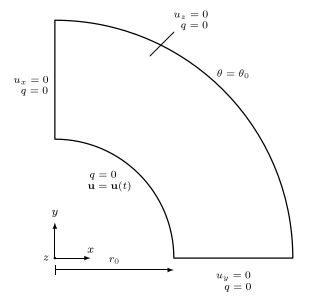
\includegraphics[width=0.5\textwidth]{problem_description}
  \caption{Boundary conditions considered in the quasi-static finite strain thermo-elastic expansion of an infinitely long thick-walled cylinder.}
\label{fig:problem_description}
\end{figure}

The decoupled Neo-Hookean free energy function shown in Equation~\ref{} characterizes the thermo-elastic material considered in this analysis, in accordance with \cite{armero_new_1992}.
% In accordance with \cite{armero_new_1992}, the following decoupled Neo-Hookean free energy function characterizes the thermo-elastic material considered in this analysis
% \[
% \hat{\Psi}=\hat{\mathrm{U}}(\mathrm{J})+\hat{\mathrm{W}}(\overline{\mathbf{C}})+\hat{\Psi}_{\Theta}(\Theta)+\hat{M}(\mathrm{~J}, \Theta)
% \]
% where the volumetric \(\hat{U}(J)\) and the isochoric \(\hat{W}(\overline{\mathbf{C}})\) part yield
% \[
% \hat{\mathrm{U}}(\mathrm{J})=\frac{\kappa}{2} \ln ^{2}(\mathrm{~J}), \quad \hat{\mathrm{W}}(\overline{\mathbf{C}})=\frac{\mu}{2}[\operatorname{tr}(\overline{\mathbf{C}})-3] .
% \]
% In addition, we choose for the thermal part
% \[
% \hat{\Psi}_{\Theta}(\Theta)=c\left[\left(\Theta-\Theta_{0}\right)-\Theta \ln \left(\Theta / \Theta_{0}\right)\right]
% \]
% resulting in a constant specific heat capacity \(c_{p}=c\) and finally assume a coupled part as
% \[
% \hat{M}(J, \Theta)=-3 \alpha\left(\Theta-\Theta_{0}\right) \frac{d \hat{U}(J)}{d J}=-3 \alpha \kappa\left(\Theta-\Theta_{0}\right) \frac{\ln (J)}{J}
% \]
% which models the assumption of purely volumetric thermal expansion; see [7]. The coupled part \(\hat{M}(\mathrm{~J}, \Theta)\) represents the thermo-mechanical coupling effects since the volumetric stress tensor reads
% \[
% \mathbf{S}_{\mathrm{vol}}(\mathbf{C}, \Theta)=\mathrm{Jp} \mathbf{C}^{-1}=\kappa\left[\ln J-3 \alpha\left(\Theta-\Theta_{0}\right) \frac{(1-\ln \mathrm{J})}{\mathrm{J}}\right] \mathbf{C}^{-1}
% \]
% where \(p=\mathrm{d} \hat{\Psi} / \mathrm{dJ}\) and the thermo-elastic coupling follows from (17):
% \[
% \mathscr{H}(\mathbf{C}, \Theta)=\Theta \frac{\partial^{2} \Psi}{\partial \mathrm{J} \partial \Theta} \mathrm{J}=-3 \alpha \kappa \Theta \frac{(1-\ln \mathrm{J})}{\mathrm{J}^{2}} \mathrm{~J}
% \]



\subsection{Validation of the Numerical Results}

To validate the results presented in this work regarding the quasi-static finite strain thermo-elastic expansion of an infinitely long thick-walled cylinder,
the problem is solved considering an \(\alpha_T = \SI{1.65e-4}{\kelvin^{-1}}\) and a \(\alpha_T = \SI{1.65e-5}{\kelvin^{-1}}\), at three different displacement rates for the inner raidus, (\(\dot u_0 = \SIlist{0.1; 0.25; 0.5}{\milli\meter\second^{-1}}\)).
Reference results for this configuration of the problem are available in \cite{ibrahimbegovic_thermodynamics_2009}, and provide a suitable comparison for the validation of the results obtained in the present work \jvc{Not sure about this}.
The values chosen for the expansion coefficient lead to, so-called, weak and strong coupling.
The use of the latter value for the thermal expansion coefficient leads to instabilities when using a fixed-point explicit or implicit schemes with the isothermic split \citep{ibrahimbegovic_thermodynamics_2009, erbts_accelerated_2012}.

The results for \(\alpha_T = \SI{1.65e-5}{\kelvin^{-1}}\) and \(\alpha_T =\SI{1.65e-4}{\kelvin^{-1}}\) are presented in Figures~\ref{fig:thick_cylinder_validation_inner_radius_temperature_weak_coupled_quad4fbar} and \ref{fig:thick_cylinder_validation_inner_radius_temperature_strong_coupled_quad4fbar}.
A good agreement between the numerical results produced in the present work an the ones found in \cite{ibrahimbegovic_thermodynamics_2009} can be observed for all displacement rates considered.

\begin{figure}
  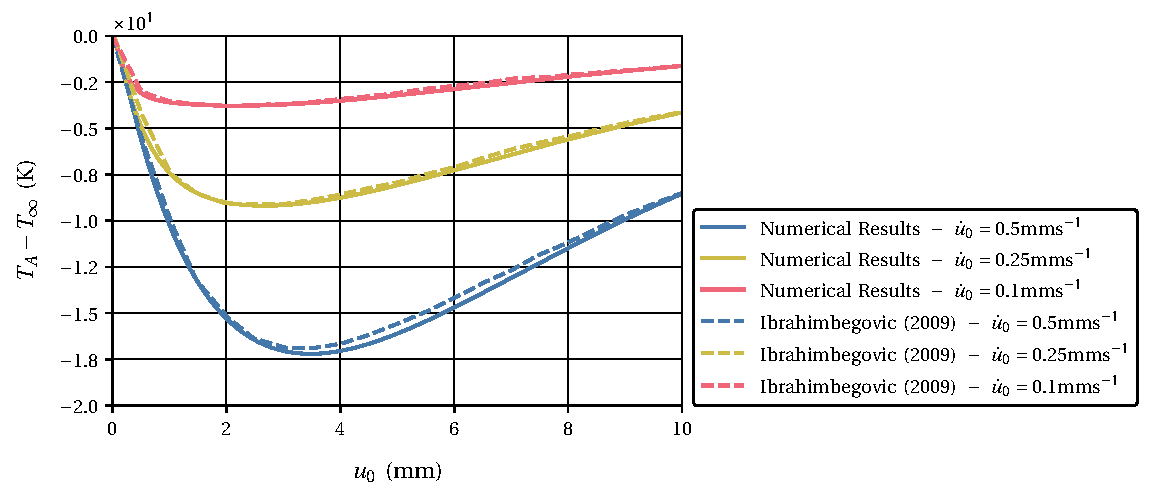
\includegraphics[width=\textwidth]{thick_cylinder_validation_inner_radius_temperature_weak_coupled_quad4fbar}
  \caption{Difference between the temperature at the inner radius and the reference temperature for the expansion of the thick-walled cylinder with \(\alpha_T=\SI{1.65e-5}{\kelvin^{-1}}\) and at different displacement rates for the inner radius (\(\dot u_0 = \SIlist{0.1; 0.25; 0.5}{\milli\meter\second^{-1}}\)}
\label{fig:thick_cylinder_validation_inner_radius_temperature_weak_coupled_quad4fbar}

\end{figure}
\begin{figure}
  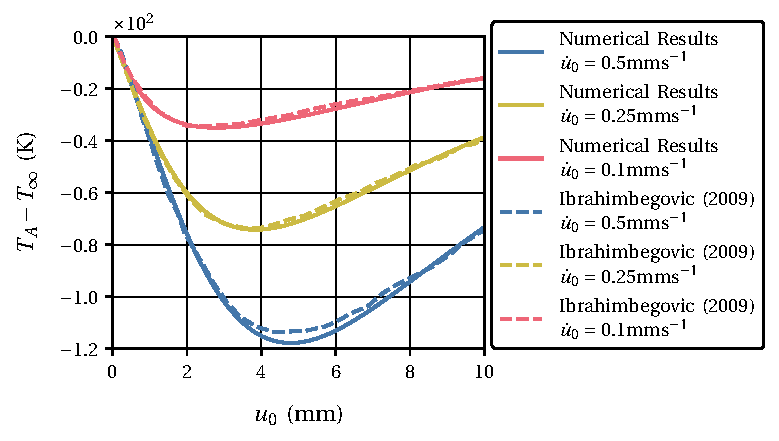
\includegraphics[width=\textwidth]{thick_cylinder_validation_inner_radius_temperature_strong_coupled_quad4fbar}
  \caption{Difference between the temperature at the inner radius and the reference temperature for the expansion of the thick-walled cylinder with \(\alpha_T=\SI{1.65e-4}{\kelvin^{-1}}\) and at different displacement rates for the inner radius (\(\dot u_0 = \SIlist{0.1; 0.25; 0.5}{\milli\meter\second^{-1}}\)}
\label{fig:thick_cylinder_validation_inner_radius_temperature_strong_coupled_quad4fbar}
\end{figure}

\subsection{Evaluation and comparison of implicit solution methods for the coupled problem}

The following contains the results concerning the evaluation and comparison of the implicit solution methods for coupled problems considered in this work.
The discussion starts with the methods that require only one evalution of the residual, implicitly requiring the solution of both the thermal and the mechanical problems by the corresponding solvers, per nonlinear iteration.
The Broyden-like family of methods fall into this category too but are considered by themselves and are presented next.
The Newton-Krylov methods are also analysed, followed by the vector extrapolation methods with cycling.
The discussion ends with the comparison bewteen the best methods of each class.

The analysis presented is based mainly on four pieces of information.
The first concerns how the residual evolves as a function of the nonlinear iterations.
The second is the number of function evaluations needed to solve the coupled problem to the desired accuracy at each time step.
The third an fourth are the total number of function evaluations and the total CPU time needed to solve the coupled problem to the desired accuracy as a function of the thermal expansion coefficient.
The larger the thermal expansion coefficient the stronger the coupling between the thermal and mechanical fields, and the harder the problem is to solve.

Only one displacement rate is considered (\(\dot u_0 = \SI{0.5}{\milli\meter\second^{-1}}\)), with the thermal expansion coefficient varying from \SI{0}{\kelvin^{-1}} to \SI{1.5e-4}{\kelvin^{-1}}.

\subsubsection{Methods with only one residual evaluation per iteration}

The methods with only one residual evaluation per iteration considered are the fixed-point method (see Section~\ref{}), underrelaxation (see Section~\ref{}), Aitken relaxation (see Section~\ref{}) and Broyden's method, Type I and II (see Section~\ref{}).
These are, a priori, the most parcimonious methods regarding residual evaluations, as only one is performed per nonlinear iteration.
The underrelaxation is performed with \(\omega = 0.5\), and the first relaxation coefficient for the Aitken relaxation is also set to 0.5.

Figure~\ref{fig:thick_cylinder_single_iter_residual_1st_time_step_quad4fbar_pred} presents the residual in percentage as a function of the number of nonlinear iterations in the first time step with \(\alpha_T=\SI{1.5e-4}{\kelvin^{-1}}\) and \(\dot u_0 =\SI{0.5}{\milli\meter\second^{-1}}\).
As reported by \cite{erbts_accelerated_2012}, the fixed-point scheme is unable to converge for this value of the thermal expansio coefficient \jvc{Confirm this}.
The other methods all converge approximately linearly, with the Broyden methods and the Aitken relaxation method taking the same number of nonlinear iterations/function evaluations.
Furthermore, the two Broyden methods are visually undistinguishable.
The underrelaxation methods takes more iterations to converge, however this could possibly be improved by further tuning of the relaxation coefficient, set in this case to 0.5.

\begin{figure}
  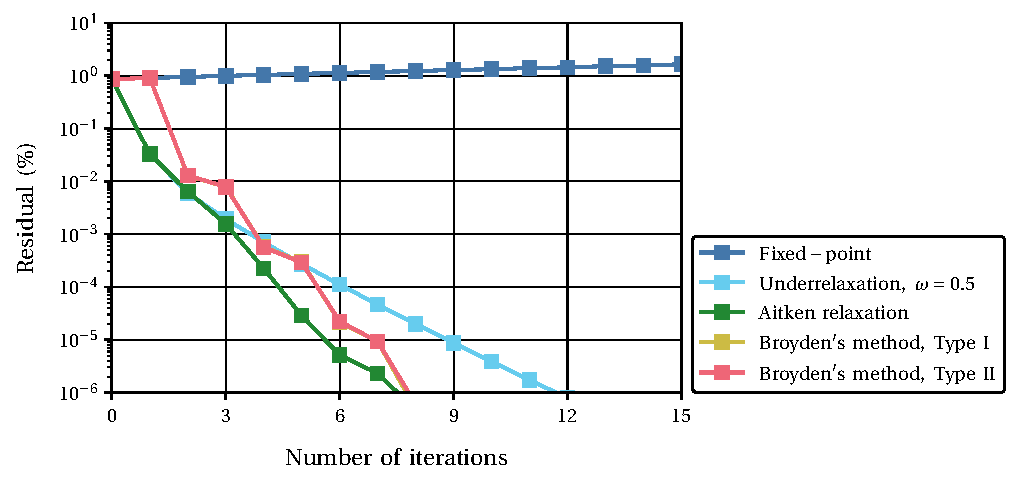
\includegraphics[width=\textwidth]{thick_cylinder_single_iter_residual_1st_time_step_quad4fbar_pred}
  \caption{Residual in percentage as a function of the number of nonlinear iterations in the first time step with \(\alpha_T=\SI{1.5e-4}{\kelvin^{-1}}\) and \(\dot u_0 =\SI{0.1}{\milli\meter\second~{-1}}\) for the implicit methods for the solution of coupled problems that perform only one evaluation per nonlinear iteration.}
\label{fig:thick_cylinder_single_iter_residual_1st_time_step_quad4fbar_pred}
\end{figure}

Figure~\ref{fig:thick_cylinder_single_iter_n_iter_time_quad4fbar_pred} presents the number of nonlinear iterations/numer of function evaluations needed to solve the coupled problem at each time step and the total (cumulative) number of iterations needed.
The strength of the coupling, tighly connected to the difficulty in solving the coupled problem and hence the number of nonlinear iterations needed to solve it, seems to be approximately uniform across the displacement range considered.
The Broyden methods show a very similar behavior that best the Aitken relaxation at each time step by at most one or two nonlinear iterations.
This leads however to a sizable difference in the total number of function evaluations needed to solve the problem from start to finish.
The underrelaxation under performs again, showing even more difficulty in solving the problem as the displacement increases.

\begin{figure}
  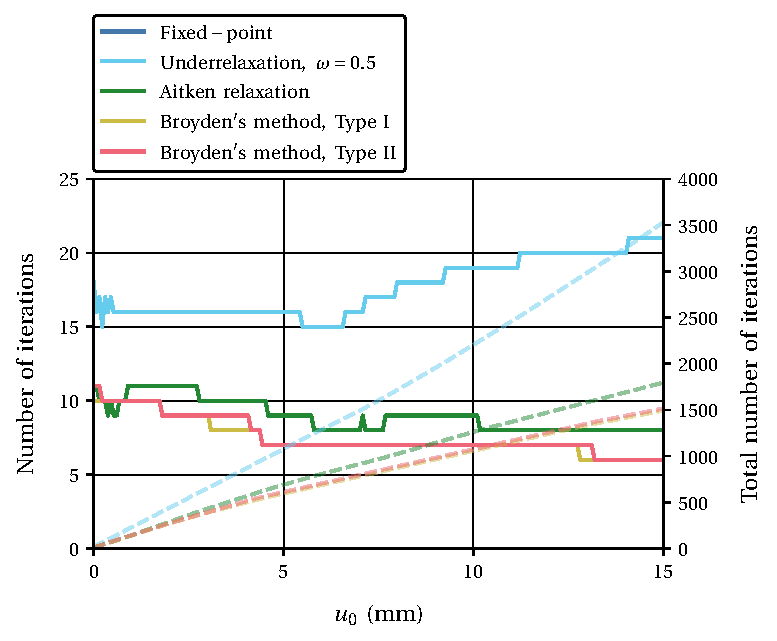
\includegraphics[width=\textwidth]{thick_cylinder_single_iter_n_iter_time_quad4fbar_pred}
  \caption{Number of nonlinear iterations needed to solve the coupled problem at each time step and the total number of iterations needed to solve the coupled problem ith \(\alpha_T=\SI{1.5e-4}{\kelvin^{-1}}\) and \(\dot u_0 =\SI{0.1}{\milli\meter\second~{-1}}\) for the implicit methods for the solution of coupled problems that perform only one evaluation per nonlinear iteration.}
\label{fig:thick_cylinder_single_iter_n_iter_time_quad4fbar_pred}
\end{figure}

Figures~\ref{fig:thick_cylinder_single_iter_n_iter_time_quad4fbar_pred} and \ref{fig:thick_cylinder_single_iter_n_iter_coupl_strength_quad4fbar_pred} present the total number of residual evaluations, in this case corresponding also to the total number of nonlinear iterations, and the total CPU time in seconds as a function of the thermal expansion coefficient, which controls the strength of the coupling between the thermal and the mechanical fields, repsectively.
It can be clearly understood that the number of residual evaluations coorelates perfectly with the total CPU time.
The most efficient methods are the two Broyden methods, followed by the Aitken relaxation.
The underrelaxation method performes poorly through out the range of values considered for the thermal expansion coefficient and the fixed-point becomes incresingly slow as the coupling gets stronger eventually failing to converge for \(\alpha_T=\SI{1.5e-4}{\kelvin^{-1}}\).

\begin{figure}
  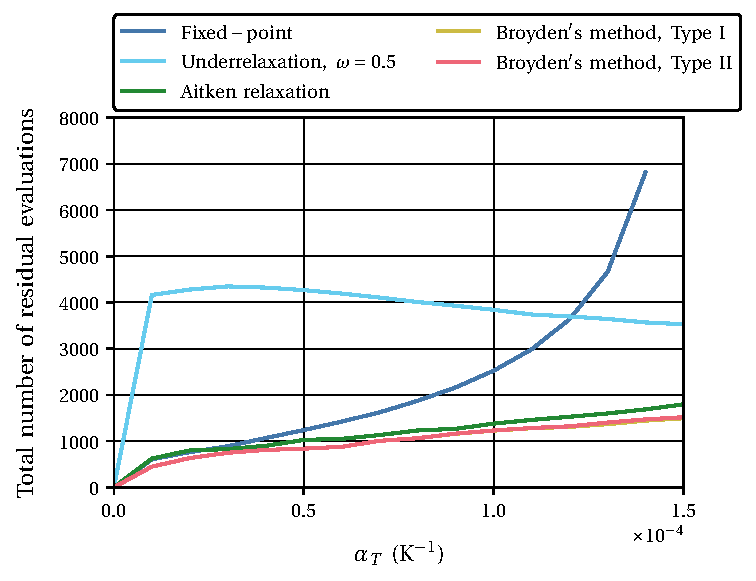
\includegraphics[width=\textwidth]{thick_cylinder_single_iter_n_iter_coupl_strength_quad4fbar_pred}
  \caption{Total number of residual evaluations as a function of the thermal expansion coefficient with \(\alpha_T=\SI{1.5e-4}{\kelvin^{-1}}\) and \(\dot u_0 =\SI{0.1}{\milli\meter\second~{-1}}\) for the implicit methods for the solution of coupled problems that perform only one evaluation per nonlinear iteration.}
\label{fig:thick_cylinder_single_iter_n_iter_coupl_strength_quad4fbar_pred}
\end{figure}

\begin{figure}
  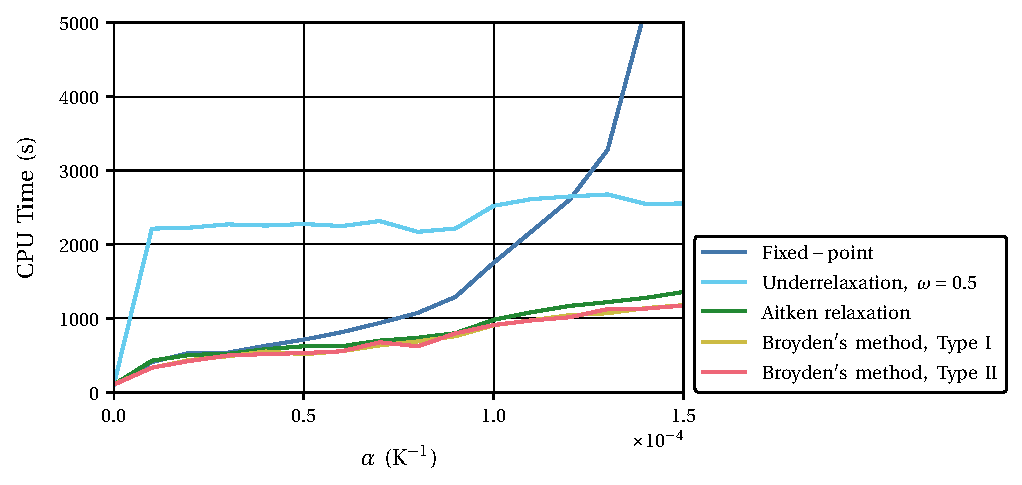
\includegraphics[width=\textwidth]{thick_cylinder_single_iter_cpu_time_coupl_strength_quad4fbar_pred}
  \caption{Total CPU time in seconds as a function of the thermal expansion coefficient with \(\alpha_T=\SI{1.5e-4}{\kelvin^{-1}}\) and \(\dot u_0 =\SI{0.1}{\milli\meter\second~{-1}}\) for the implicit methods for the solution of coupled problems that perform only one evaluation per nonlinear iteration.}
\label{fig:thick_cylinder_single_iter_cpu_time_coupl_strength_quad4fbar_pred}
\end{figure}

\jvc{write a small conclusion!!!}

\subsection{Broyden-like method}

The Broyden-like methods considered are possess update groups \(s=1,\ 2,\ 3,\ 6\) with a maximum memory equal to 6.
The mixing parameters considered are \(\beta=-1,\ \num{2e-3},\ \num{2e-2}\).
All combinations are also considered with both Type I and Type II updating.

Figures~\ref{fig:thick_cylinder_broyden_like_type_i_residual_1st_time_step_quad4fbar_pred} and \ref{thick_cylinder_broyden_like_type_ii_residual_1st_time_step_quad4fbar_pred} present the residual in percentage as a function of the number of nonlinear iterations in the first time step with \(\alpha_T=\SI{1.5e-4}{\kelvin^{-1}}\) and \(\dot u_0 =\SI{0.5}{\milli\meter\second^{-1}}\) for Broyden-like methods with Type I and Type II updates, respectively.
There is no marked difference bewteen methods that employ a Type I and Type II update.
However, the choice for the mixing parameter and the number of grouping used for the input and output deltas leads to different behaviors for the residual.
For \(\beta=-1\), the methods using \(s=1\), 2 and 3 behave much the same, and are the ones needing the fewest iterations to reach the desired accuracy.
For \(s=6\) the residual behaves differently, plateuaing during the evaluation of the function.
Despite this, it doesn't take a much larger number of iterations.
The cases with \(\beta=\num{2e-3}\) and \num{2e-2} exihibt a similar trend, with plateuas not justified in the same.
Despite this weird behavior they converge all the same.
The choice of \(\beta=\num{2e-2}\) seems to lead to slightly fewer iterations before the desired accuracy is reached.

\begin{figure}
  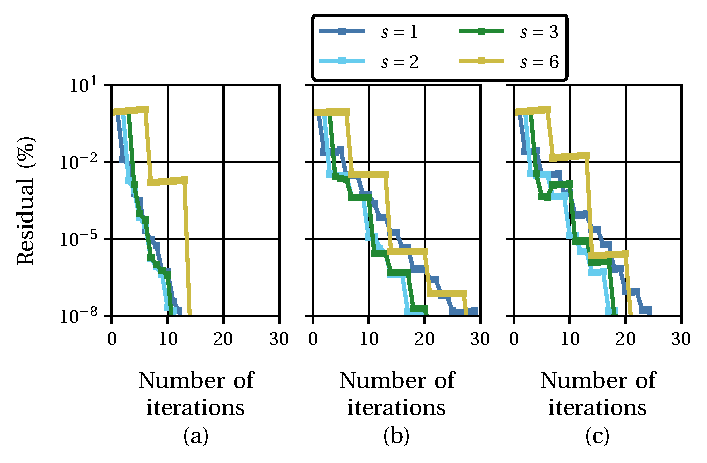
\includegraphics[width=.9\textwidth]{thick_cylinder_broyden_like_type_i_residual_1st_time_step_quad4fbar_pred}
  \caption{Residual in percentage as a function of the number of nonlinear iterations in the first time step with \(\alpha_T=\SI{1.5e-4}{\kelvin^{-1}}\) and \(\dot u_0 =\SI{0.1}{\milli\meter\second^{-1}}\) for Broyden-like methods with Type I update and group sizes \(s=1\), 2, 4 and 6: (a) \(\beta=-1\), (b) \(\beta=\num{2e-3}\), and (c) \(\beta=\num{2e-2}\).}
\label{fig:thick_cylinder_broyden_like_type_i_residual_1st_time_step_quad4fbar_pred}
\end{figure}

\begin{figure}
  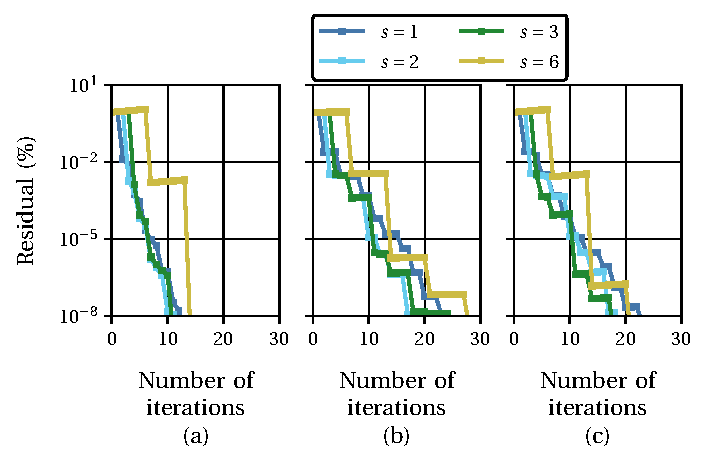
\includegraphics[width=.9\textwidth]{thick_cylinder_broyden_like_type_ii_residual_1st_time_step_quad4fbar_pred}
  \caption{Residual in percentage as a function of the number of nonlinear iterations in the first time step with \(\alpha_T=\SI{1.5e-4}{\kelvin^{-1}}\) and \(\dot u_0 =\SI{0.1}{\milli\meter\second^{-1}}\) for Broyden-like methods with Type II update and group sizes \(s=1\), 2, 4 and 6: (a) \(\beta=-1\), (b) \(\beta=\num{2e-3}\), and (c) \(\beta=\num{2e-2}\).}
\label{fig:thick_cylinder_broyden_like_type_ii_residual_1st_time_step_quad4fbar_pred}
\end{figure}

Figures~\ref{fig:thick_cylinder_broyden_like_type_i_n_iter_time_quad4fbar_pred} and \ref{fig:thick_cylinder_broyden_like_type_ii_n_iter_time_quad4fbar_pred} presents the number of nonlinear iterations/number of function evaluations needed to solve the coupled problem at each time step and the total (cumulative) number of iterations needed.
Again the differences bewteen the Broyde-like methods using Type I and Type II updates is not very strong.
Perhaps the most apparent difference is verified for the \(\beta\) values \num{2e-3} and \num{2e-2}, where the total number of iterations needed to solve the coupled thermomechanical problem for the Type I methods oscillates much more between time steps.
For \(\beta=-1\), the methods using group sizes of 1, 2 and 3 display a higher efficiency, which disappears as the displacement increases.
For \(\beta=\num{2e-2}\) and \num{2e-3}, the results seem to indicate the need for fewer iterations when using group sizes of 2 and 3.

\begin{figure}
  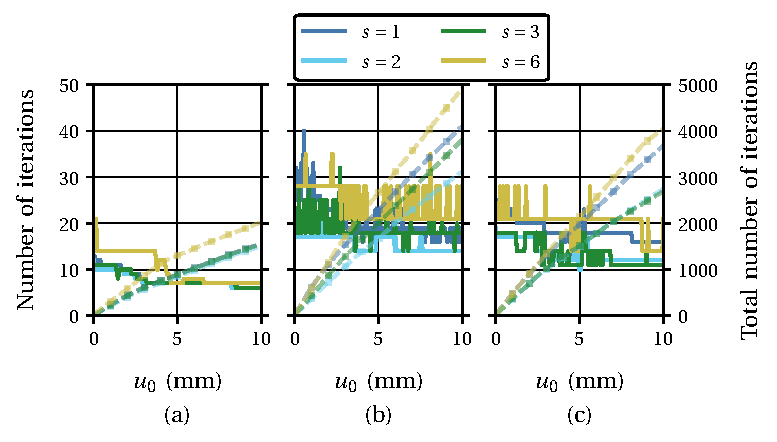
\includegraphics[width=\textwidth]{thick_cylinder_broyden_like_type_i_n_iter_time_quad4fbar_pred}
  \caption{Number of nonlinear iterations needed to solve the coupled problem at each time step and the total number of iterations needed to solve the coupled problem ith \(\alpha_T=\SI{1.5e-4}{\kelvin^{-1}}\) and \(\dot u_0 =\SI{0.1}{\milli\meter\second~{-1}}\) for Broyden-like methods with Type I update and group sizes \(s=1\), 2, 4 and 6: (a) \(\beta=-1\), (b) \(\beta=\num{2e-3}\), and (c) \(\beta=\num{2e-2}\).}
\label{thick_cylinder_broyden_like_type_i_n_iter_time_quad4fbar_pred}
\end{figure}

\begin{figure}
  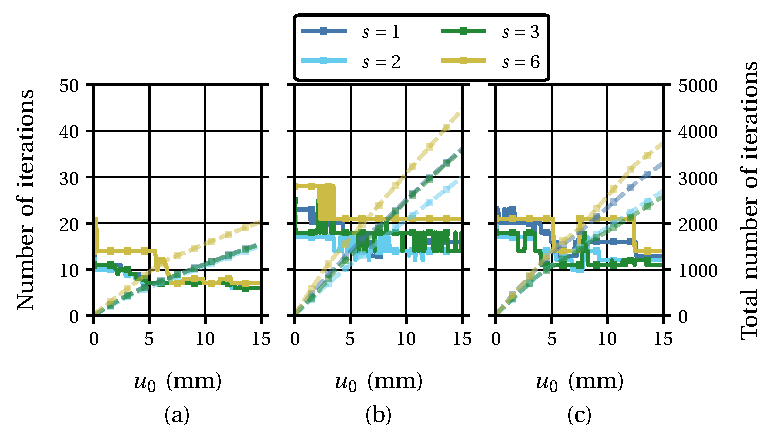
\includegraphics[width=\textwidth]{thick_cylinder_broyden_like_type_ii_n_iter_time_quad4fbar_pred}
  \caption{Number of nonlinear iterations needed to solve the coupled problem at each time step and the total number of iterations needed to solve the coupled problem ith \(\alpha_T=\SI{1.5e-4}{\kelvin^{-1}}\) and \(\dot u_0 =\SI{0.1}{\milli\meter\second~{-1}}\) for Broyden-like methods with Type II update and group sizes \(s=1\), 2, 4 and 6: (a) \(\beta=-1\), (b) \(\beta=\num{2e-3}\), and (c) \(\beta=\num{2e-2}\).}
\label{fig:thick_cylinder_broyden_like_type_ii_n_iter_time_quad4fbar_pred}
\end{figure}

Figures~\ref{fig:thick_cylinder_broyden_like_type_i_n_iter_coupl_strength_quad4fbar_pred} and \ref{fig:thick_cylinder_broyden_like_type_i_n_iter_coupl_strength_quad4fbar_pred} present the total number of residual evaluations and the total CPU time in seconds as a function of the thermal expansion coefficient, repsectively, for the Broyden-like methods with Type I update considere.
The same results are presented in Figures~\ref{thick_cylinder_broyden_like_type_ii_n_iter_coupl_strength_quad4fbar_pred} and \ref{thick_cylinder_broyden_like_type_ii_cpu_time_coupl_strength_quad4fbar_pred} for the Broyden-like methos with Type II update.
Again, it can be clearly understood that the number of residual evaluations coorelates perfectly with the total CPU time.
The most efficient methods are the methods using a mixing parameter equal to \(\beta=-1\) and group sizes equal to 1, 2 and 3.
The choices of \num{2e-3} and \num{2e-2} for the mixing parameter lead to less efficient methods, which need a larger amount of residual evaluations and thus require more CPU time to solve the coupled thermomechanical problem completly.

\begin{figure}
  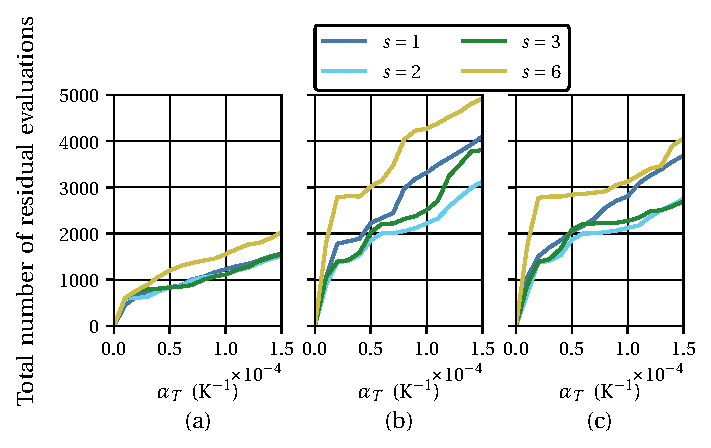
\includegraphics[width=.9\textwidth]{thick_cylinder_broyden_like_type_i_n_iter_coupl_strength_quad4fbar_pred}
  \caption{Total number of residual evaluations as a function of the thermal expansion coefficient with \(\alpha_T=\SI{1.5e-4}{\kelvin^{-1}}\) and \(\dot u_0 =\SI{0.1}{\milli\meter\second~{-1}}\) for the implicit methods for Broyden-like methods with Type I update and group sizes \(s=1\), 2, 4 and 6: (a) \(\beta=-1\), (b) \(\beta=\num{2e-3}\), and (c) \(\beta=\num{2e-2}\).}
\label{fig:thick_cylinder_broyden_like_type_i_n_iter_coupl_strength_quad4fbar_pred}
\end{figure}

\begin{figure}
  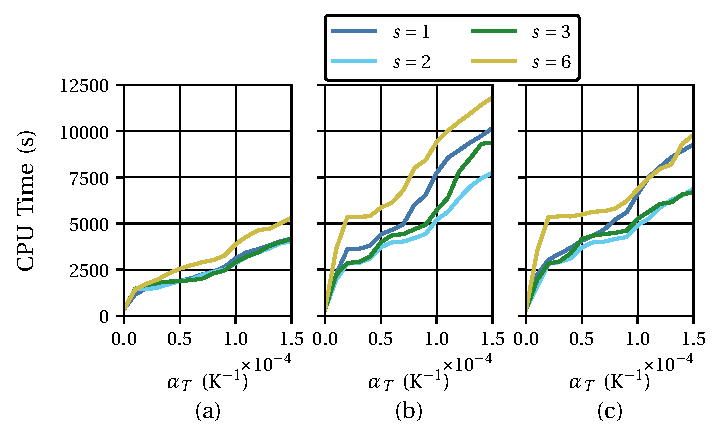
\includegraphics[width=.9\textwidth]{thick_cylinder_broyden_like_type_i_cpu_time_coupl_strength_quad4fbar_pred}
  \caption{Total CPU time in seconds as a function of the thermal expansion coefficient with \(\alpha_T=\SI{1.5e-4}{\kelvin^{-1}}\) and \(\dot u_0 =\SI{0.1}{\milli\meter\second~{-1}}\) for Broyden-like methods with Type I update and group sizes \(s=1\), 2, 4 and 6: (a) \(\beta=-1\), (b) \(\beta=\num{2e-3}\), and (c) \(\beta=\num{2e-2}\).}
\label{fig:thick_cylinder_broyden_like_type_i_cpu_time_coupl_strength_quad4fbar_pred}
\end{figure}

\begin{figure}
  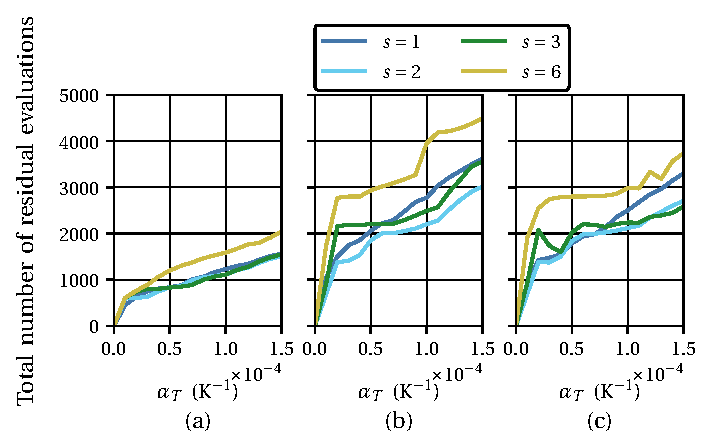
\includegraphics[width=.9\textwidth]{thick_cylinder_broyden_like_type_ii_n_iter_coupl_strength_quad4fbar_pred}
  \caption{Total number of residual evaluations as a function of the thermal expansion coefficient with \(\alpha_T=\SI{1.5e-4}{\kelvin^{-1}}\) and \(\dot u_0 =\SI{0.1}{\milli\meter\second~{-1}}\) for Broyden-like methods with Type II update and group sizes \(s=1\), 2, 4 and 6: (a) \(\beta=-1\), (b) \(\beta=\num{2e-3}\), and (c) \(\beta=\num{2e-2}\).}
\label{fig:thick_cylinder_broyden_like_type_ii_n_iter_coupl_strength_quad4fbar_pred}
\end{figure}

\begin{figure}
  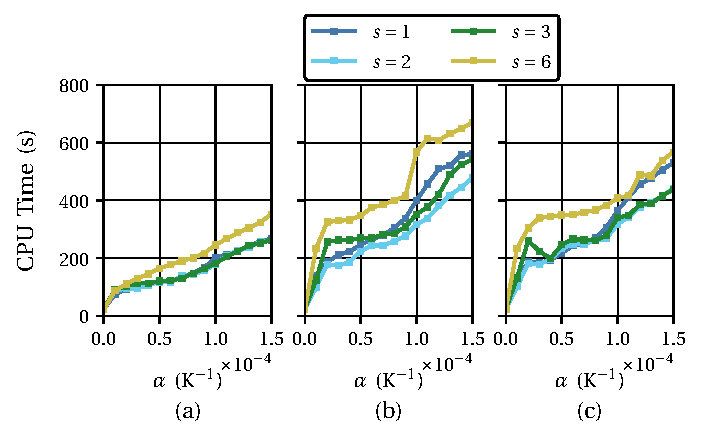
\includegraphics[width=.9\textwidth]{thick_cylinder_broyden_like_type_ii_cpu_time_coupl_strength_quad4fbar_pred}
  \caption{Total CPU time in seconds as a function of the thermal expansion coefficient with \(\alpha_T=\SI{1.5e-4}{\kelvin^{-1}}\) and \(\dot u_0 =\SI{0.1}{\milli\meter\second~{-1}}\) for Broyden-like methods with Type II update and group sizes \(s=1\), 2, 4 and 6: (a) \(\beta=-1\), (b) \(\beta=\num{2e-3}\), and (c) \(\beta=\num{2e-2}\).}
\label{fig:thick_cylinder_broyden_like_type_ii_cpu_time_coupl_strength_quad4fbar_pred}
\end{figure}


\subsection{Newton-GMRES method}

\subsection{Polynomial vector extrapolation with cycling}\jvc{Check if the name is not the other way around}

\subsection{Comparison for the best methods}

\begin{figure}
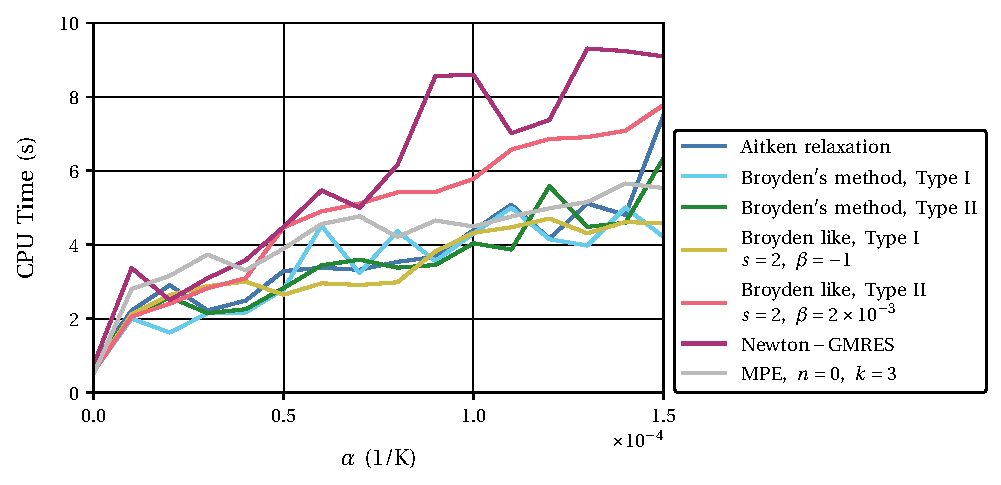
\includegraphics[width=\textwidth]{thick_cylinder_comparison_methods_best_cpu_time_coupl_strength_quad4fbar_pred}
\end{figure}

\begin{figure}
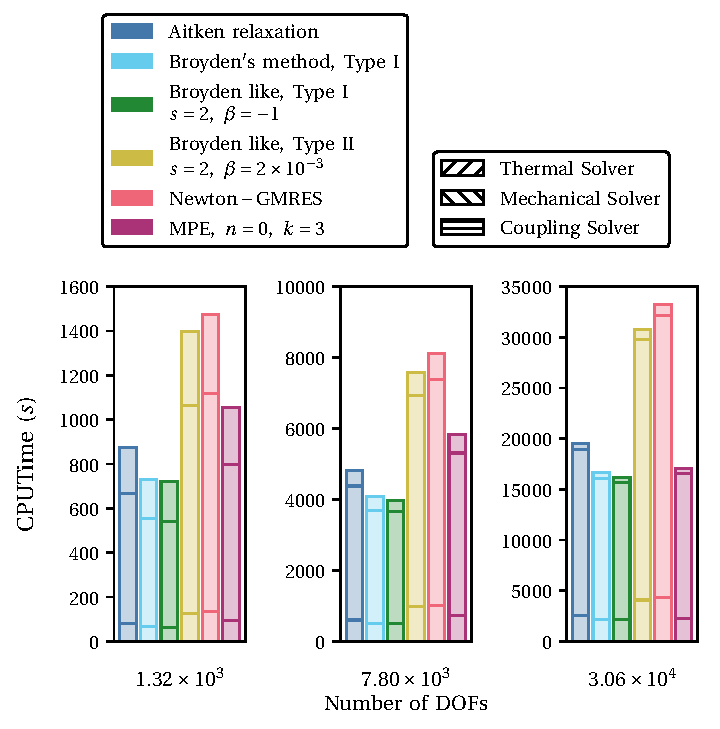
\includegraphics[width=\textwidth]{thick_cylinder_comparison_methods_best_time_profile_mesh_size_quad4fbar_pred}
\end{figure}

% \begin{table}
%   \centering
%   \caption{Material properties, and initial and boundary conditions for the problem concerning the expansion of a thick-walled cylinder.}
%   \label{tab:snd_danilovskaya_description}
%   \begin{tabular}{c
%     S[exponent-mode=engineering]
%     S[exponent-mode=engineering]
%     S[exponent-mode=engineering]
%     S[exponent-mode=engineering]
%     S[exponent-mode=engineering]
%     S[exponent-mode=engineering]}
%   $\Delta t$ \si{\second} & {\multicolumn{3}{c}{0.1}} & {\multicolumn{3}{c}{1.0}}\\
%   $\alpha$ \SI{1e-5}{\kelvin^{-1}} & {5} & {10} & {15} & {5} & {10} & {15}\\
%   \hline\hline
%   \hline\hline
%   \end{tabular}
% \end{table}

\subsection{Mechanically driven problem: necking of a circular bar}
\label{sec:mech-driv-probl}

The first validation example consists of the thermally triggered necking of a circular bar, as originally reported in \cite{simo1992AssociativeCoupledThermoplasticity} and repeated in \cite{danowski2014ComputationalModellingThermoStructure}.
The problem consists of a cylindrical bar of radius $r=\SI{6.413}{\milli\meter}$ and length $h=\SI{53.334}{\milli\meter}$ subjected to a prescribed axial displacement $\bar{u}_{y}=\SI{8}{\milli\meter}$ at both ends during $t=\SI{8}{\second}$.
The supports at the tips allow transverse contraction of the specimen.
The bar is initially at the environment temperature $T_{0}=T_{\infty}=\SI{293}{\kelvin}$ and is subjected to heat transfer by convection at all boundaries, with the heat transfer coefficient $h_{c} = \SI{17.5e-3}{\newton\per\milli\meter\per\second\per\kelvin}$.
The material is modelled with the constitutive model by \cite{simo1992AssociativeCoupledThermoplasticity} and the material properties are given in \ref{tab:matpropsnecking}.
%
\begin{table}[!tb]
  \caption{Material properties used in the circular bar necking example.}
  \label{tab:matpropsnecking}
  \centering
  \begin{tabular}{@{}lccc@{}}
    \toprule
    Property & Symbol & Value & Units  \\ \midrule
    Bulk modulus & $K $ & \SI{164206}{} & \si{\newton\per\milli\meter\squared} \\
    Coefficient of thermal expansion & $\alpha_{T} $ & \SI{1e-5}{} & \si{\per\kelvin} \\
    Density & $\rho_{0} $ & \SI{7.8e-9}{} & \si{\newton\second\squared\per\milli\meter\tothe{4}} \\
    Dissipation factor  & $\chi $ & \SI{0.9}{} & - \\
    Initial yield stress at $T_{0}$ & $\sigma_{y,0} $ & \SI{450}{} & \si{\newton\per\milli\meter\squared} \\
    Linear hardening coefficient at $T_{0}$ & $H $ & \SI{129.24}{} & \si{\newton\per\milli\meter\squared} \\
    Reference temperature  & $T_{0} $ & \SI{293}{} & \si{\kelvin} \\
    Saturation exponent & $\delta $ & \SI{16.93}{} & - \\
    Saturation yield stress at $T_{0}$ & $\sigma_{y,\infty} $ & \SI{715}{} & \si{\newton\per\milli\meter\squared} \\
    Shear modulus & $\mu $ & \SI{80193.8}{} & \si{\newton\per\milli\meter\squared} \\
    Specific heat & $C_V$ & \SI{0.46e9}{} & \si{\milli\meter\squared\per\second\squared\per\kelvin} \\
    Thermal conductivity & $k_{0} $ & \SI{45}{} & \si{\newton\per\second\per\kelvin} \\
    Thermal softening parameter ($\sigma_{y,0}$) & $\omega_{0} $ & \SI{0.002}{} & \si{\per\kelvin} \\
    Thermal softening parameter ($\sigma_{y,\infty}$, $H$) & $\omega_{h} $ & \SI{0.002}{} & \si{\per\kelvin} \\ \bottomrule
  \end{tabular}
\end{table}
%
This is a classical benchmark in isothermal elastoplasticity, that renders a bifurcation problem where the necking phenomenon is typically triggered by a geometric imperfection.
In the thermomechanical version, the combination of plastic dissipation in the bulk and the heat transfer at the boundaries produce a temperature field that becomes progressively more heterogeneous during the loading.
With growing elongation, the temperature rise in the centre of the bar will increase relative to the exterior boundary and automatically triggers the necking, even in a geometrically perfect setup.

The problem is analysed using two-dimensional axisymmetric, reduced integration QUAD8 elements and three-dimensional HEXA8-FBAR elements \cite{desouzaneto1996DesignSimpleLow} for the mechanical problem, and standard fully integrated elements for the thermal field.
\ref{fig:necking} illustrates the problem setup, the finite element mesh employed in the 2D simulations and characteristic stages of deformation and temperature field during the prescribed elongation, evidencing the significant necking of the bar.
%
\begin{figure}[p]
  \centering
  % \def\svgwidth{1.0\linewidth}
  % \footnotesize
  % \input{necking.pdf_tex}
  \caption{Description of the thermally triggered necking of a circular bar problem, characteristic deformation and temperature field stages during the loading and example axisymmetric finite element mesh. The results represented have been obtained with reduced integration QUAD8 elements, non-adiabatic boundary conditions, the inconsistent mechanical dissipation formulation and the Fourier law based on constant $k_{0}$.}
  \label{fig:necking}
\end{figure}
%
Only one-quarter of the specimen is simulated, resulting in a finite element mesh with 1141 nodes and 450 elements for the 2D case and  3937 nodes and 3240 elements for the 3D counterpart.
The load is applied in 80 equal time steps $\Delta t = \SI{0.1}{\second}$.
A quasi-static solution is computed for the mechanical problem using a Backward-Euler integration and the transient temperature field is integrated in time with the Generalised-$\alpha$ method with $\rho_{\infty,T}=1.0$.
The coupled solution is determined using the explicit coupling algorithm, solving the mechanical problem first and the thermal problem second.

The results are validated by comparing the reaction force at the supports and the neck surface temperature at point A, see \ref{fig:necking}.
Different reference data is included in the analysis, in particular, the adiabatic and non-adiabatic results presented in the original work by \cite{simo1992AssociativeCoupledThermoplasticity} and the non-adiabatic results presented in \cite{danowski2014ComputationalModellingThermoStructure}.
It should be remarked that there are five fundamental differences between these two publications that lead to distinct results.
First, in \cite{simo1992AssociativeCoupledThermoplasticity}, the authors adopt a mechanical dissipation term that is thermodynamically inconsistent, based on the previously mentioned dissipation factor, $\chi$, whereas, in \cite{danowski2014ComputationalModellingThermoStructure}, the authors use the mechanical dissipation coming directly from the second law of thermodynamics.
Second, \cite{danowski2014ComputationalModellingThermoStructure} also uses a consistent structural heating term for the Gough-Joule effect, accounting for both elastic and plastic contributions.
In contrast, \cite{simo1992AssociativeCoupledThermoplasticity} considered the elastic contributions, exclusively.
For more information on the previous classification and mathematical formulas for the heating parcels, the reader is referred to \ref{cha:simo-miehes-thermo}.
The third difference is linked to the heat conduction law employed in each contribution.
Although the large deformation version of the Fourier law underlies both publications, \cite{simo1992AssociativeCoupledThermoplasticity} considered as a fixed material parameter the spatial thermal conductivity, $k$, and in \cite{danowski2014ComputationalModellingThermoStructure}, the material thermal conductivity, $k_{0}$, was instead interpreted as the fixed material parameter.
Without further mention, the latter is employed in the current work.
Fourth, \cite{simo1992AssociativeCoupledThermoplasticity} solved the coupled problem using an operator split scheme and \cite{danowski2014ComputationalModellingThermoStructure} pursued a monolithic solution.
Last, regarding  spatial discretisation, \cite{danowski2014ComputationalModellingThermoStructure} used HEXA8-FBAR elements and \cite{simo1992AssociativeCoupledThermoplasticity} employed mixed displacement-pressure QUAD8 elements.

To enable a fair comparison with the reference data, the numerical solution is calculated using both the adiabatic and non-adiabatic setups.
Furthermore, in the latter, the consistent and inconsistent interpretations are considered, including a calculation with fixed $k$.
The evolution of the reaction force and neck surface temperature as a function of the prescribed displacement are shown in \ref{fig:necking-results} for the 2D and 3D solutions, respectively.
\begin{figure}[!p]
  \centering
  % \includegraphics[width=1.0\linewidth]{./solution-techniques-thermomechanics/figures/necking/necking_results.pdf}
  \caption{Evolution of the reaction force at the tips of the bar and the neck surface temperature with the prescribed displacement using QUAD8 elements with reduced integration (QUAD8R) and HEXA8-FBAR elements.}
  \label{fig:necking-results}
\end{figure}
%
From a physical interpretation standpoint, the plot of reaction forces suggests that the simulation occurs almost entirely in the elastoplastic regime.
The necking process does not occur in the isothermal and adiabatic solutions, with the adiabatic solution predicting slightly smaller reactions due to the thermal softening effect.
Also, in this case, the temperature evolves uniformly in the bar and grows in a nearly linear fashion over time, as captured in the numerical solutions.
As previously postulated, the necking is automatically triggered in the non-adiabatic solutions, which produces a heavy reduction in the reaction force starting approximately at $\bar{u}_{y}=\SI{4}{\milli\meter}$, followed by a steep temperature rise due to the higher plastic dissipation.

Inspecting \ref{fig:necking-results} from a validation perspective, the numerical results show a good agreement with the literature.
The correlation between the non-adiabatic, inconsistent solution and fixed $k$ with the results from \cite{simo1992AssociativeCoupledThermoplasticity} is very satisfactory, both on the temperature and the reaction force side.
Curiously, while the reaction force seems almost insensitive to the element type employed, the neck temperature is better approximated with the QUAD8 solution, especially near the maximum displacement.
The slight difference observed between these cases can presumably be attributed to the distinct element technology and coupling solution strategy used to obtain the two curves.
Relative to the solutions based on the consistent mechanical heating, the numerical results show good agreement with the curves extracted from \cite{danowski2014ComputationalModellingThermoStructure} up to $\bar{u}_{y}=\SI{3}{\milli\meter}$, but features significant differences from there on, both in the mechanical and thermal responses.
The results are still consistent insofar as the numerical solution obtained in this solution predicts a smaller temperature increase but larger reaction forces, as the thermal softening is less pronounced.
Unfortunately, to the author's knowledge, there are no other bibliographical sources that consider the fully consistent thermomechanical version of the model to support any of the sides.
Nevertheless, as the accuracy relative to the results from \cite{simo1992AssociativeCoupledThermoplasticity} is already adequate, the possibly remaining issue resides at the constitutive model level and therefore does not compromise the coupling environment.
It should also be remarked that if the prescribed displacement is slightly larger, the weakly coupled partitioned solution diverges at some point.
This can be expected from the mathematical properties associated with this type of strategy, as discussed in this chapter.
In truth, numerical divergence can be observed to start near $\bar{u}_{y}=\SI{8}{\milli\meter}$ for the non-adiabatic, inconsistent solution, see \ref{fig:necking-results}.
In principle, it is possible to stabilise the solution by employing more advanced techniques, for instance, implicit coupling strategies with numerical acceleration.
Despite being paramount for a robust computer simulation tool, these topics are postponed to future developments.
Overall, the present results are a sound indication of the correct implementation of the coupling environment, in particular, the data exchange and solution orchestration.
\begin{figure}
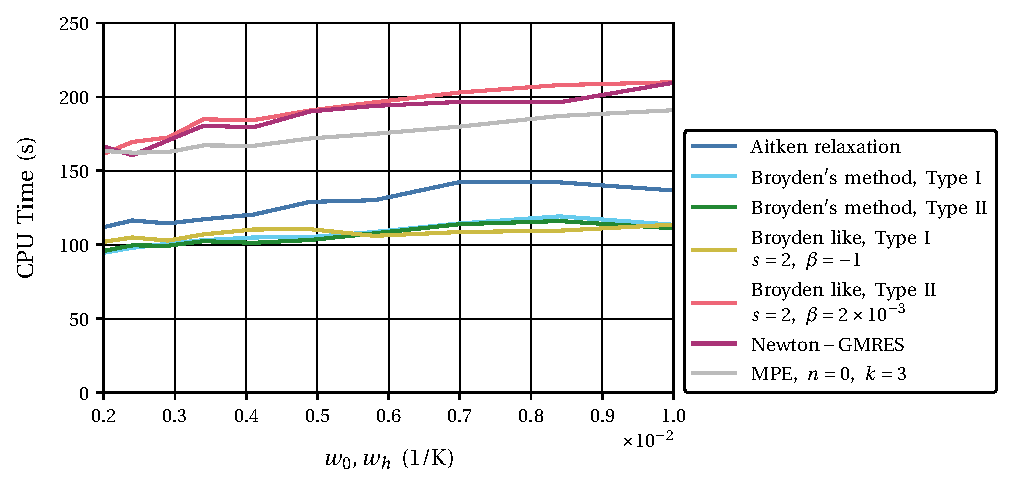
\includegraphics[width=\textwidth]{necking_comparison_methods_best_cpu_time_coupl_strength_quad4fbar_pred}
\end{figure}

\begin{figure}
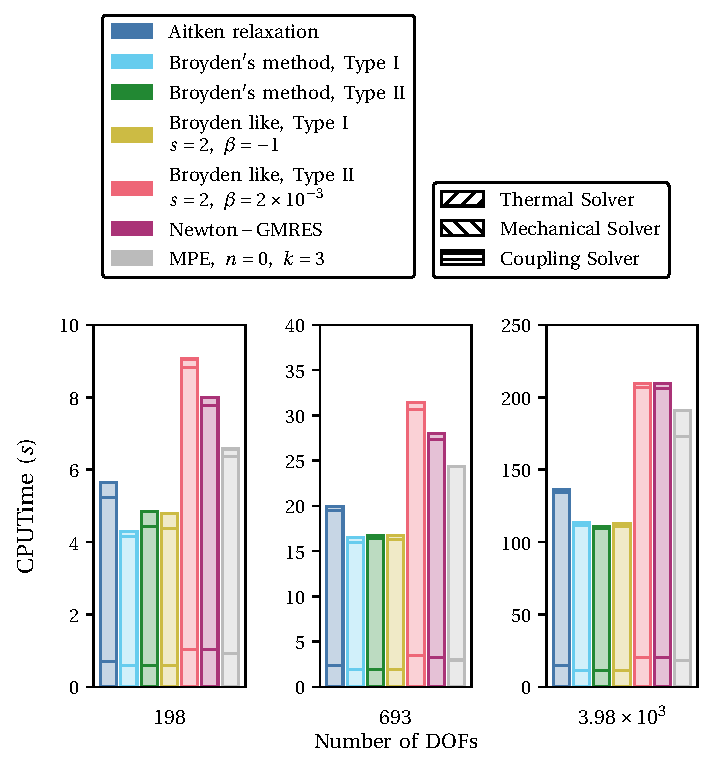
\includegraphics[width=\textwidth]{necking_comparison_methods_best_time_profile_mesh_size_quad4fbar_pred}
\end{figure}
